
\subsection{Voorpagina}\label{voorpagina}

De voorpagina

\subsubsection{Grid}

De template van de website bestaat uit een grid, een soort geraamte. Het grid is opgebouwd uit verschillende regio's. In elke regio kunnen blokken geplaatst worden. In de paragraaf \emph{Felix}\see{felix}  staat beschreven hoe en welke je blokken kunt toevoegen aan een regio. 

\bigskip

\begin{center}
	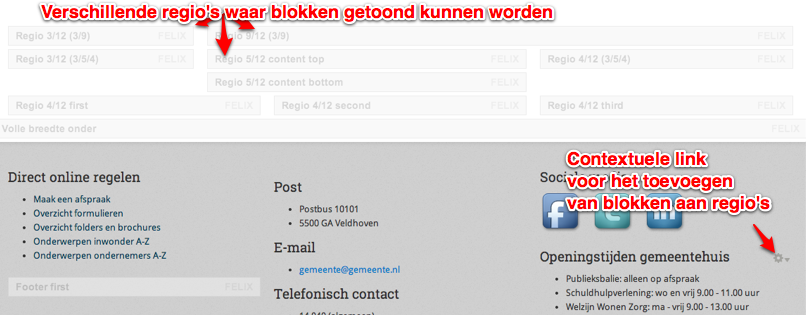
\includegraphics[width=\textwidth]{img/grid1.png}
\end{center}


\subsubsection{Blokken}

In de onderstaande afbeeldingen worden alle bestaande blokken op voorpagina in het kort toegelicht.

\bigskip

\begin{center}
	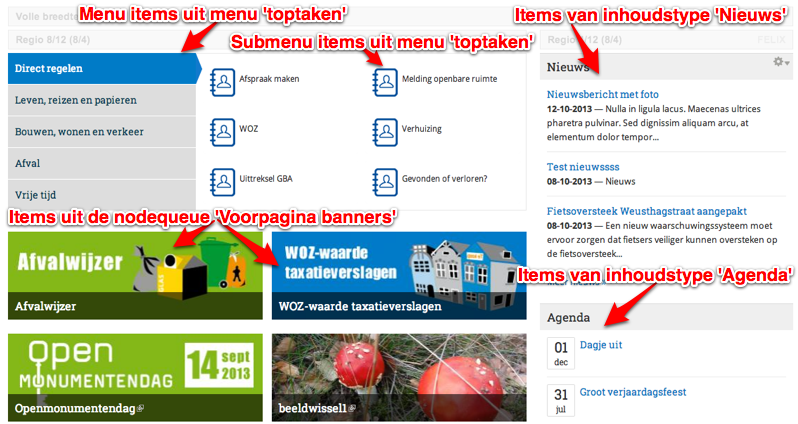
\includegraphics[width=\textwidth]{img/voorpagina1.png}

	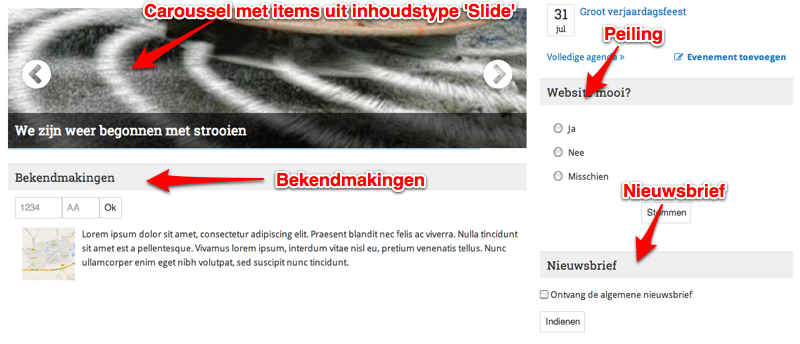
\includegraphics[width=\textwidth]{img/voorpagina2.png}

	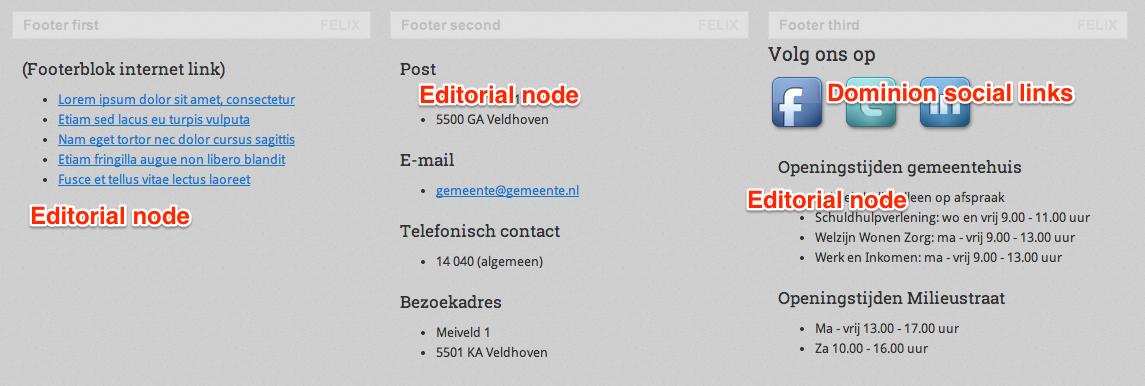
\includegraphics[width=\textwidth]{img/voorpagina3.png}
\end{center}
